\documentclass{article}
\usepackage[a4paper, left=2cm, right=2cm, top=3cm, bottom=3cm, headheight=35pt, includehead]{geometry}

\usepackage[english]{babel}
\usepackage[utf8]{inputenc}
\usepackage{fancyhdr}

\usepackage{enumitem}
\usepackage{amsmath}
\usepackage{mathtools}
\usepackage{listings}


\usepackage{tikz}
\usetikzlibrary{arrows.meta}


\lstset{mathescape=true,
		morekeywords={if,else,and,then,for,return}}

\pagestyle{fancy}
\fancyhf{}
\lhead{\today \\ Andrés Montoya, 405409 \\ Laura Koch, 406310 }
\chead{Introduction to Artificial Intelligence \\ Assignment 02}
\rhead{ Lennart Holzenkamp, 407761 \\ Simon Michau, 406133 \\ Til Mohr, 405959}

\begin{document}

\section*{Exercise 2.1}
\begin{enumerate}[label=(\alph*)]
	\item	$g(n)$ denotes the path cost from the root of the search tree to node $n$. Since the Greedy Search always expands the node $n^*$ where $h(n^*) = g(n^*)$ is minimal, the resulting algorithm can be described as a shortest path search (or lowest cost search) algorithm.
	\item	Since $d(n)$ denotes the depth of a node $n$ in the search tree and the Greedy Search always expands the node $n^*$ where $h(n^*) = d(n^*)$ is minimal (so minimal depth), the resulting algorithm is a BFS.
	\item	$\frac{1}{1+d(n)}$ is inversely proportional to the depth of node $n$ in the search tree. Therefore, the Greedy Search always expands the node $n^*$ with the largest depth. So we get an DFS algorithm.
\end{enumerate}

\section*{Exercise 2.2}
\subsection*{1)}
An admissible heuristic is a function that never overestimates the cost of the minimum cost path from a node to the goal node. Let $h^*(n)$ be the optimal cost to reach the goal from $n$. If $h$ is admissible, then $\forall n: h(n) \leq h^*(n)$.\\[2\baselineskip]
Let $h$ be consistent.\\
Suppose there is not path from $n$ to the goal state. Then $h^*(n) = \infty$, therefore $h(n) \leq h^*(n)$.\\
Now suppose that there is some path from $n$ to te goal state $g$. Let $(n, x_1, \dots, x_m, g)$ be the shortest path from $n$ to the goal state $g$ with corresponding actions $(a_n, a_{x_1}, \dots, a_{x_m})$.\\[2\baselineskip]
Induction:\\
Consider $x_m$. $h(x_m) \leq c(x_m, a_{x_m}, g) + h(g) \stackrel{h(g)=0}{=} c(x_m, a_{x_m}, g) = h^*(x_m)$.\\
Similarly $x_{m-1}$. $h(x_{m-1}) \leq c(x_{m-1}, a_{x_{m-1}}, x_m) + h(x_m) = c(x_{m-1}, a_{x_{m-1}}, x_m) + c(x_m, a_{x_m}, g) = h^*(x_{m-1})$.\\
By induction on the shortest past we get $h(n) \leq c(n, a_n, x_1)+ c(x_m, a_{x_m}, g) = h^*(n)$, which is of course the shortest path cost.\\[2\baselineskip]
Therefore when a heuristic is consistent, it is admissible.

\subsection*{2)}
Let there be the graph with goal node $G$:

\begin{figure}[htb]
\begin{minipage}[c]{.49\textwidth}
	\centering
	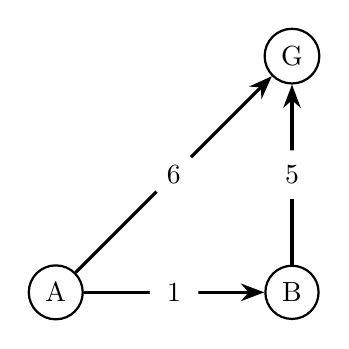
\begin{tikzpicture}
		\begin{scope}[every node/.style={circle,thick,draw}]
			\node (A) at (0,0) {A};
			\node (B) at (3,0) {B};
			\node (G) at (3,3) {G};
		\end{scope}

		\begin{scope}[>={Stealth[black]},
					every node/.style={fill=white,circle},
					every edge/.style={draw=black,very thick}]
			\path [->] (A) edge node {$1$} (B);
			\path [->] (B) edge node {$5$} (G);
			\path [->] (A) edge node {$6$} (G);
		\end{scope}
	\end{tikzpicture}
\end{minipage}
\begin{minipage}[c]{.49\textwidth}
	\centering
	\begin{tabular}{c|c}
		Node $n$ & $h^*(n)$ \\
		\hline
		A & 6 \\
		B & 5 \\
		G & 0
	\end{tabular}
\end{minipage}
\end{figure}

An admissible heuristic, that is not consistent:

\begin{center}
	\begin{tabular}{c|c}
		Node $n$ & $h(n)$ \\
		\hline
		A & 6 \\
		B & 1 \\
		G & 0
	\end{tabular}
\end{center}

\section*{Exercise 2.3}


\section*{Exercise 2.4}
\begin{enumerate}[label=(\alph*)]
	\item	First we create a search graph
			\begin{itemize}
				\item	States/Nodes $V$: $(j_1,j_2) \in \{0,1,2,3\} \times \{0,1,2,3,4\}$\\
						A state $(j_i, j_2)$ reflects how much liter of water is in jug $1$ and jug $2$.
				\item	Actions $A \coloneqq \{f_i, e_i, p_{i,j} \vert i,j \in \{1,2\} \land i \neq j\}$\\
						$f_i$ denotes the action of filling jug $i$. $e_i$ denotes the action of emptying jug $i$. $p_{i,j}$ denotes the action of pouring all the possible water from jug $i$ into jug $j$.
				\item	Edges $E \subseteq V \times V$: $(v_1, v_2, a) \in V \times V \times A$
						Each edge (directed) $(v_1, v_2, a)$ denotes a change of state $v_1$ into $v_2$ by action $a$.\\
						There should only be possible edges in our graph: (the restrictions prevent self loops)
						\begin{itemize}
							\item	$((j_1, j_2), (3, j_2), f_1)$, if $j_1 \neq 3$
							\item	$((j_1, j_2), (j_1, 4), f_2)$, if $j_2 \neq 4$
							\item	$((j_1, j_2), (0, j_2), e_1)$, if $j_1 \neq 0$
							\item	$((j_1, j_2), (j_1, 0), e_2)$, if $j_2 \neq 0$
							\item	$((j_1, j_2), (\max(0, j_1 - \min(3, 4-j_2)), j_2 + (j_1 - \max(0, j_1 - \min(3, 4-j_2))), p_{1,2})$, if $j_1 \neq 0 \land j_2 \neq 4$
							\item	$((j_1, j_2), (j_1 + (j_2 - \max(0, j_2 - (3 - j_1)))), \max(0, j_2 - (3 - j_1))), p_{2,1})$, if $j_2 \neq 0 \land j_1 \neq 3$
						\end{itemize}
			\end{itemize}

			Now we can search from starting position $(0,0)$ to goal position $(0,2)$ in this graph.
		\item	\begin{center}
					\begin{tabular}{c|c||c|c}
						$j_1$ & $j_2$ & $h(n)$ & reason \\
						\hline
						$*$ & $2$ & 0 & given (final) \\
						$0$ & $0$ & 5 & given \\
						$0$ & $0<y\neq 2$ & y & given \\
						$3$ & $y<4\neq 2$ & 3 & given \\
						$3$ & $4$ & 5 & given \\
						$0<x<3$ & $y<4\neq 2$ & 4 & $f_1$ \\
						$0<x<3$ & $4$ & 5 & $e_1$
					\end{tabular}
				\end{center}
		\item	Node Encoding: $(j_1, j_2, f)$
				\begin{center}
					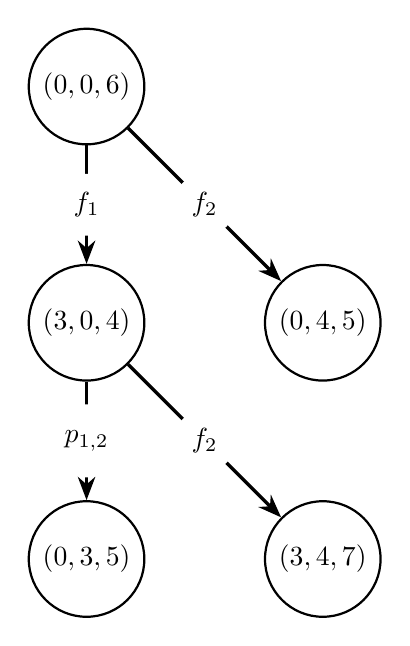
\begin{tikzpicture}
						\begin{scope}[every node/.style={circle,thick,draw}]
							% internal note encoding: j_1|j_2|layer
							% layer 0
							\node (000) at (0,0) {$(0,0,6)$};
							% layer 1
							\node (301) at (0,-3) {$(3,0,4)$};
							\node (041) at (3,-3) {$(0,4,5)$};
							% layer 2
							\node (032) at (0,-6) {$(0,3,5)$};
							\node (342) at (3,-6) {$(3,4,7)$};
							% layer 3
						\end{scope}

						\begin{scope}[>={Stealth[black]},
									every node/.style={fill=white,circle},
									every edge/.style={draw=black,very thick}]
							\path [->] (000) edge node {$f_1$} (301);
							\path [->] (000) edge node {$f_2$} (041);

							\path [->] (301) edge node {$p_{1,2}$} (032);
							\path [->] (301) edge node {$f_2$} (342);
						\end{scope}
					\end{tikzpicture}
					TODO NOT DONE YET
				\end{center}
\end{enumerate}

\end{document}